\documentclass[a4paper, 12pt]{article}

\usepackage[utf8]{inputenc}
\usepackage[T1]{fontenc}
\usepackage{lmodern}
\usepackage[german]{babel}
\usepackage{helvet}
\renewcommand{\familydefault}{\sfdefault}
\usepackage[singlespacing]{setspace}
\usepackage[margin=1in]{geometry}
\usepackage{parskip}
\usepackage{bibgerm}
\usepackage{graphicx}
\usepackage{tcolorbox}
\usepackage{dingbat}
\usepackage{pdfpages}
\usepackage{hyperref}
\usepackage{cite}
\usepackage[authoryear]{natbib}
\hypersetup{
  ,colorlinks=true
  ,linkcolor=black
  ,citecolor=black
  ,filecolor=black
  ,urlcolor=black
  }

\newcommand{\leadingzero}[1]{\ifnum #1<10 0\the#1\else\the#1\fi}
\newcommand{\datumVonHeute}{\leadingzero{\day}.\leadingzero{\month}.\the\year}

\newcommand{\Thema}{Vergleichende Untersuchung von GraphQL und REST, hinsichtlich Anpassungsfähigkeit und Leistungsfähigkeit}
\newcommand{\Autor}{Robin Hefner}
\newcommand{\Matrikelnummer}{206488}
\newcommand{\DeckblattTextEins}{Exposé}


\title{\Thema}
\author{\Autor}
\date{\today}


\begin{document}

\begin{titlepage}
\begin{figure}[hbtp]
	\centering
	
\includegraphics[scale=0.075]{img/logo.jpg}
\end{figure}
\begin{center}
\vspace{1.5cm}
{\scshape\large \DeckblattTextEins \par}
\vspace{1cm}
{\scshape\large zum Thema\par}
\vspace{1.5cm}
{\LARGE\bfseries \Thema \par}
\vfill
\vfill
{Erstellt von:\\ {\bfseries \Autor}\\ \Matrikelnummer\\ \par}
\vspace{1cm}
\end{center}
\end{titlepage}

\section{Problemstellung}
In der modernen Softwareentwicklung spielen APIs (Application Programming Interfaces) eine entscheidende Rolle bei der Integration und Kommunikation zwischen verschiedenen Diensten und Anwendungen. Traditionell wurde REST (Representational State Transfer) als Standard für die Erstellung und Nutzung von APIs verwendet. Mit der Einführung und
zunehmenden Verbreitung von GraphQL, einer Abfragesprache für APIs, die von Facebook entwickelt wurde, stehen Entwickler nun vor der Wahl zwischen diesen beiden Ansätzen. Die Wahl zwischen REST und GraphQL hat signifikante Auswirkungen auf die Entwicklung und den Betrieb der Anwendung. Unternehmen müssen eine fundierte Entscheidung treffen, welche Technologie besser zu ihren Anforderungen, im Hinblick auf Leistungsfähigkeit und Flexibilität, passt.

\section{Stand der Technik}
REST ist eine Architektur, die 2000 zum ersten Mal in einer Dissertation von Roy Fielding beschrieben wurde. Sie integriert das HTTP-Protokoll und nutzt als zentrales Element die Ressourcenorientierung, bei der jede Entität als Ressource betrachtet und durch eine eindeutige URL identifiziert wird. Die CRUD-Operationen (Create, Read, Update, Delete) werden mithilfe der HTTP-Methoden (POST, GET, PUT, DELETE) repräsentiert. Ein besonderes Merkmal ist die Zustandslosigkeit, bei der jeder API-Aufruf alle notwendigen Informationen enthält, um diesen zu bearbeiten. Hierdurch wird die Client-Server-Interaktion vereinfacht. Zudem nutzt REST das in HTTP integrierte Caching um Antwortzeiten und Leistung zu verbessern. \citep{Fielding2000}  \citep{graphqlreplacerest}


GraphQL wurde 2012 von Facebook für den internen Gebrauch entwickelt. 2015 wurde es als Open Source Projekt für die Allgemeinheit veröffentlicht. Das Herzstück von GraphQL stellen die client-getriebenen Abfragen dar, bei denen der Client die Struktur der Daten genau spezifizieren kann und nur die benötigten Daten erhält. Hierdurch werden überflüssige Datenübertragungen reduziert und effizientere Netzwerkaufrufe ermöglicht. Durch eine hierarchische Struktur der Abfragen, die die Graph-Struktur widerspiegelt, wird eine intuitive Datenmodellierung ermöglicht. Die starke Typisierung in GraphQL wird durch ein Schema definiert, dass die Typen der Daten spezifiziert und somit eine bessere Validierung und Dokumentation ermöglicht. Im Gegensatz zu REST, das für verschiedene Operationen mehrere Endpunkte benötigt, verwendet GraphQL einen einzigen Endpoint für alle API-Abfragen.  \citep{graphql}   \citep{graphqlreplacerest}
\newpage
\section{Forschungsfrage}
Diese Arbeit soll auf den Folgenden zwei Forschungsfragen basieren. \newline
Erstens, wie unterscheiden sich GraphQL und REST hinsichtlich der Anfrage- und Antwortzeiten unter verschiedenen Lastbedingungen und Anfragekomplexitäten? Diese Frage zielt darauf ab, die Performance beider Systeme unter variablen Bedingungen zu vergleichen. Beispielsweise könnte untersucht werden, wie schnell eine API auf eine einfache Datenabfrage reagiert, im Vergleich zu einer komplexeren, die mehrere Abhängigkeiten involviert. Diese Untersuchung könnte Einblicke in die Effizienz der beiden Technologien bieten und somit als Entscheidungshilfe für Entwickler dienen, die die beste Lösung für ihre spezifischen Bedürfnisse auswählen möchten.


Zweitens stellt sich die Frage, inwiefern bieten GraphQL und REST unterschiedliche Möglichkeiten zur Abfrageanpassung? Diese Frage beleuchtet die Flexibilität beider Systeme in Bezug auf die Individualisierung von Datenabfragen. Während REST traditionell durch feste Endpunkte gekennzeichnet ist, die jeweils eine bestimmte Datenstruktur zurückgeben, bietet GraphQL eine dynamischere Herangehensweise. Mit GraphQL können Clients genau die Daten anfordern, die sie benötigen, und keine zusätzlichen Informationen, was zu effizienteren Datenübertragungen führen kann. Diese Fähigkeit, Anfragen präzise anzupassen, könnte die Effizienz und Benutzerfreundlichkeit von Webanwendungen erheblich beeinflussen.


Insgesamt bieten diese beiden Forschungsfragen einen umfassenden Rahmen, um die Vor- und Nachteile von GraphQL und REST eingehend zu untersuchen. Durch die Analyse der Antwortzeiten, sowie der Möglichkeiten der Abfrageanpassung können Entwickler fundierte Entscheidungen treffen und die für Ihre Anforderung optimale Technologie wählen.
\section{Methodik}
Für die Untersuchung werden sowohl theoretische Analysen als auch empirische Experimente durchgeführt. Im Rahmen der theoretischen Analyse erfolgt eine umfassende Literaturrecherche und die Analyse bestehender Studien zur Leistungsfähigkeit und Flexibilität von REST und GraphQL. Die empirischen Experimente umfassen die Implementierung von Beispiel-APIs mit beiden Technologien sowie die Durchführung von Leistungstests. Die Leistungstests konzentrieren sich auf das Messen der Latenz bei verschiedenen Abfrageszenarien.
\newpage
\section{Vorläufige Gliederung}
\textbf{1. Abstract}
\newline
\textbf{2. Einleitung}
\newline
\textbf{3. Theoretische Grundlagen}
\newline \hspace*{10mm}
3.1 API-Grundlagen
\newline \hspace*{10mm}
3.2 REST
\newline \hspace*{10mm}
3.3 GraphQL
\newline
\textbf{4. Implementierung}
\newline \hspace*{10mm}
4.1  Aufbauen einer Testumgebung
\newline \hspace*{10mm}
4.2 Durchführen von Performance-Tests
\newline
\textbf{5. Methodik}
\newline
\textbf{6. Ergebnisse}
\newline
\textbf{7. Diskussion}
\newline
\textbf{8. Fazit}
\section{Vorläufiger Zeitplan}
\begin{figure}[hbtp]
	\centering
	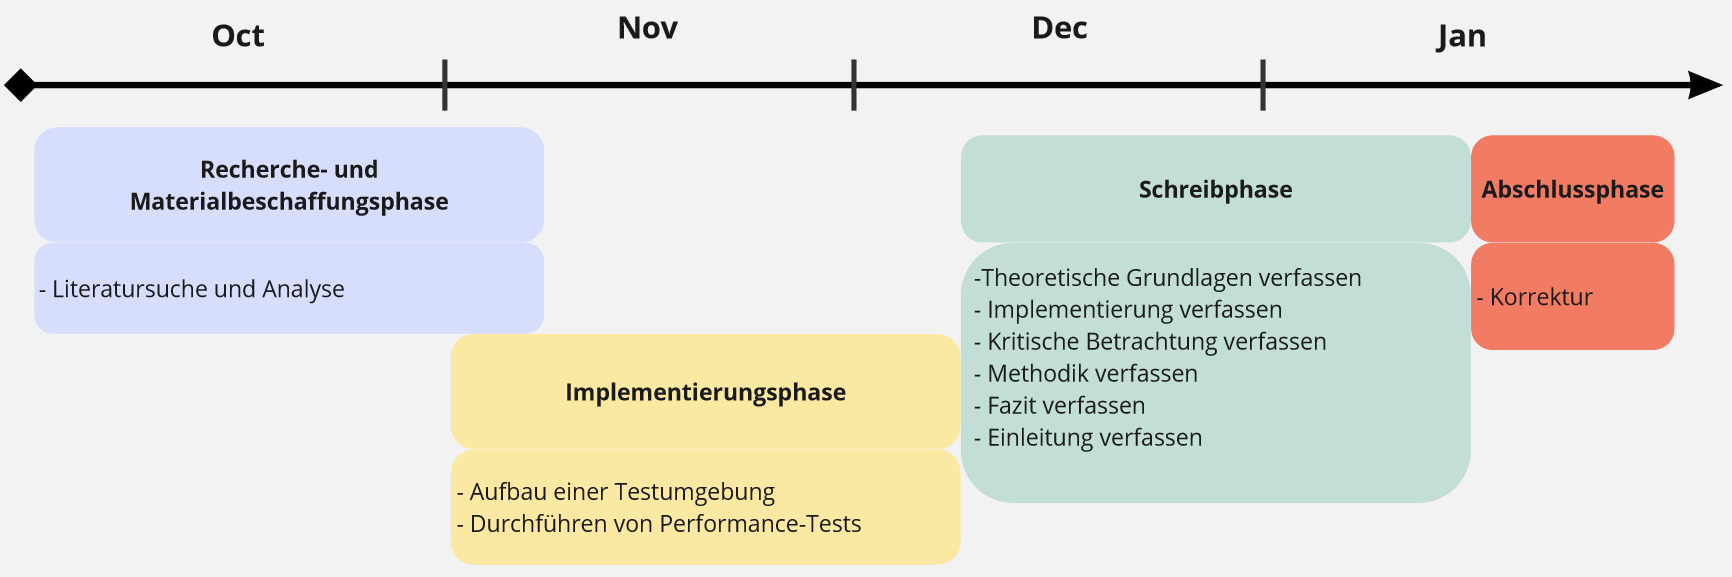
\includegraphics[scale=0.25]{img/Timeline Template.jpg}
\end{figure}

\bibliographystyle{dcu}
\bibliography{literatur}

\end{document}




